\documentclass[crop,tikz]{standalone}
\usetikzlibrary{backgrounds}
\colorlet{blue}{cyan}
\tikzset{
  inverted/.style = {
    color=white,
    background rectangle/.style={fill},
    show background rectangle
  }
}

\usepackage[european]{circuitikz}

\begin{document}
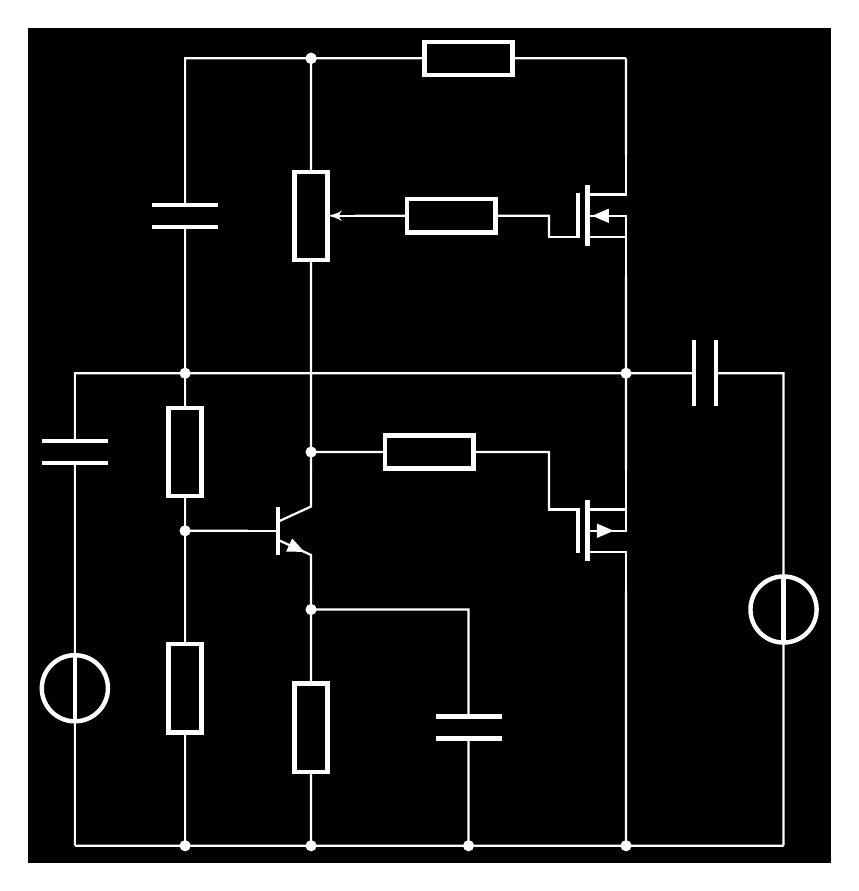
\begin{tikzpicture}[inverted,scale=2]
  \draw[thick]
    (1.5,0) to (6,0)
    (1.5,2) to[V] (1.5,0)
    (1.5,2) to[C] (1.5,3) -| (5,3)
    (2.2,2) to[R] (2.2,3)
    (2.2,2) to[red] (2.6,2)
    (2.2,3) to[C, *-] (2.2,5) -| (3,5)
    (3,0) to[R,*-*] (3,1.5) to[Tnpn,n=npn1] (3,2.5)
    (4,0) to[C, *-] (4, 1.5)--(3,1.5)
    (2.2,0) to[R, *-*] (2.2,2)
    (3,2.5) to node[short] {} (3,3)
    (3,5) to[pR, n=pot1, *-] (3,3)
    (3,5) to[R, *-] (5,5)
    (5,3) to[Tnigfetd,n=mos1] (5,5)
    (pot1.wiper) to[R] (4.5,4) -| (mos1.G)
    (5,1.5) to[Tpigfetd,n=mos2] (5,2.5)
    (5,0) to[short,*-] (mos2.D)
    (3,2.5) to[R, *-] (4.5,2.5) -| (mos2.G)
    (5,3) to[C,*-] (6,3) to[V] (6,0)
    (mos1.S)--(mos2.S)
    ;
\end{tikzpicture}
\end{document}
